\chapter{基于观测器的非线性多智能体系统间歇一致性控制}
\section{引言}
一致性问题,作为多智能体系统协调控制的基本问题,近些年来受到众多领域专家学者的关注。一致性问题是指设计合适的分布式控制协议使得多个智能体就某个共同兴趣点达成一致的问题。一致性是多智能体系统协调完成任务的前提,与群集、编队等许多问题密切相关,是最基础的也是近几十年来研究者们持续关注的问题,并且取得了大量优秀的成果。\scite{ran2007comprehensive}。
测试引用参考文献\cite{ran2007comprehensive}\scite{ran2007comprehensive,bloemen2002optimizing,breder1954equations,ding2010distributed,dunbar2006distributed,fiedler1973algebraic,gazi2003stability,ji2005connectedness,6166430,milgram1967small,olfati2006flocking,ren2007multi,vicsek1995novel,watts1998collective,zhang2008ultrafast}.
\begin{figure}[!htbp]%[!htbp]是为了固定图片的位置
\centering
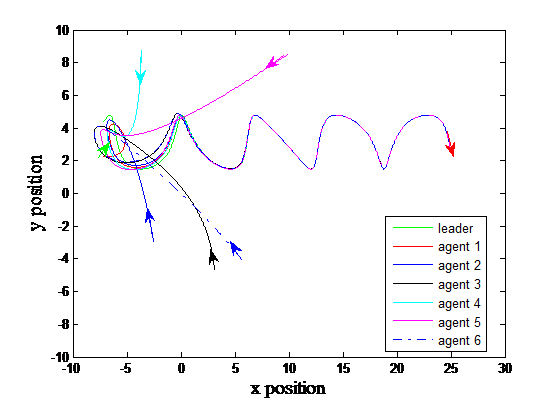
\includegraphics[width=0.8\textwidth]{5.png}
\caption{切换拓扑下多智能体系统的轨迹}
\end{figure}
\begin{Theorem}
测试
\end{Theorem}
\begin{Theorem}
测试
\end{Theorem}
\begin{Theorem}
测试
\end{Theorem}
\begin{Lemma}
测试引理
\end{Lemma}
\begin{Lemma}
测试引理
\end{Lemma}
\begin{Remark}
测试标注,“注”是楷体加粗,然后注的内容是宋体。
\end{Remark}
\setcounter{Theorem}{0}
\begin{Example}
测试例子,“例”是楷体加粗,然后例子的内容是宋体。
\end{Example}
\begin{Example}
测试例子
\end{Example}
